\chapter{
  High Luminosity LHC and High Granularity Calorimeter Upgrade
 }\label{ch_hgcal}

About \gls{HL-LHC} \gls{HGCAL} Upgrade

\section{
  Technical Design
 }

\begin{figure}[!ht]
  \centering
  \begin{minipage}[c]{0.49\textwidth}
    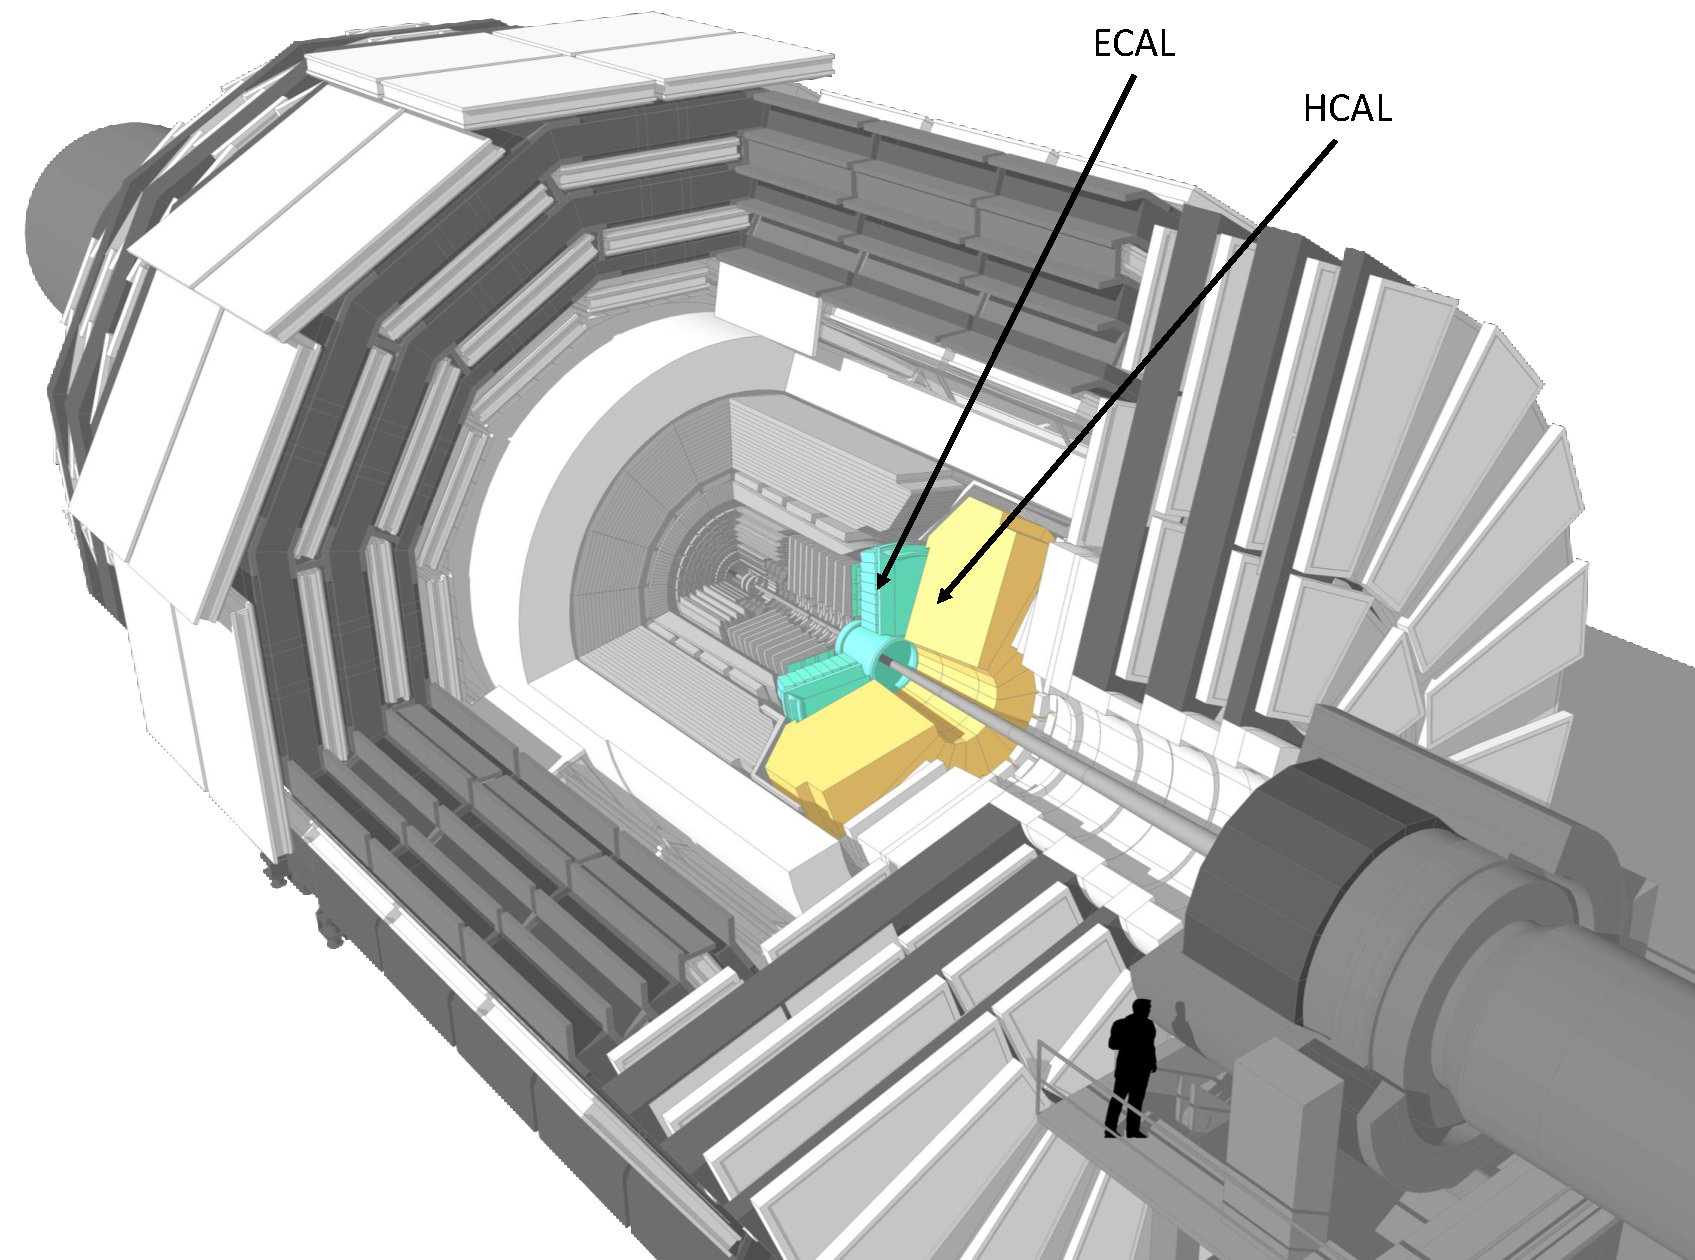
\includegraphics[width=\textwidth]{figures/hgcal/hgcal_place.pdf}
  \end{minipage}
  \begin{minipage}[c]{0.49\textwidth}
    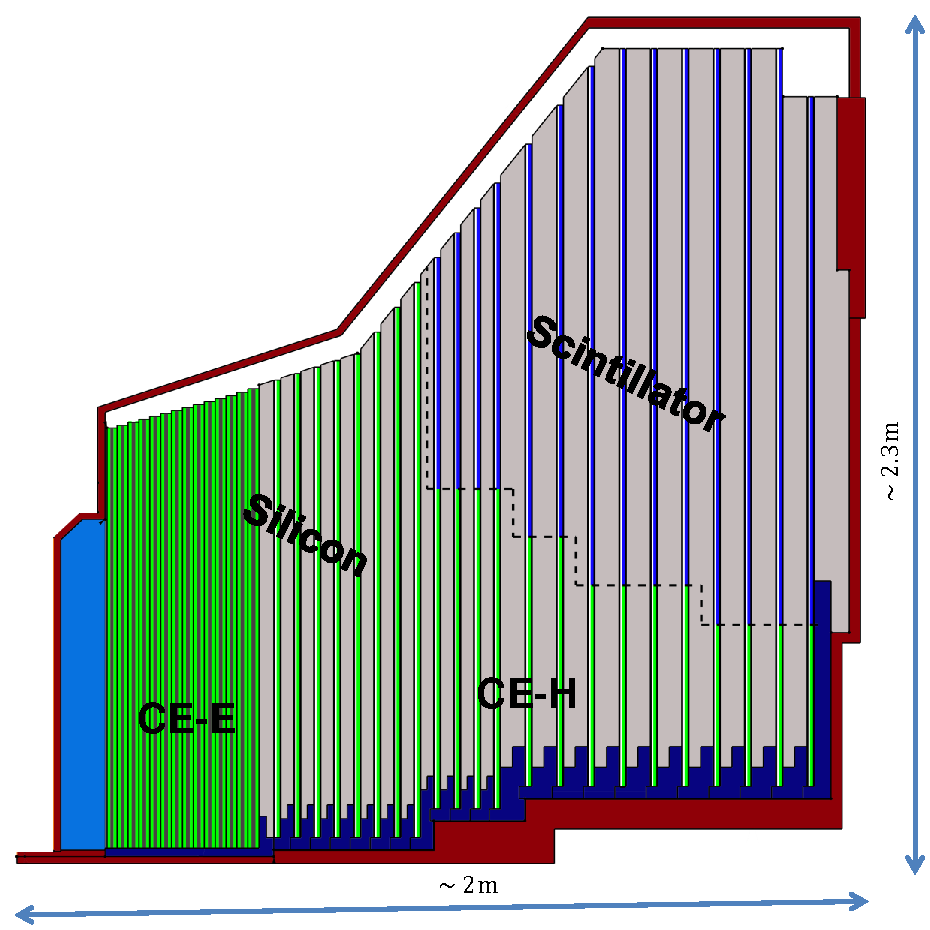
\includegraphics[width=0.9\textwidth]{figures/hgcal/hgcal_quadrant.pdf}
  \end{minipage}
  \caption[Overview of CE]%
  {Overview of CE~\cite{image-cms-hgcal-quadrant-layout,image-cms-hgcal-place}}%
  \label{fig:cms-hgcal-quadrant-layout}
\end{figure}

\section{
  Scintillator Tiles
 }

%\begin{figure}[!ht]
%  \centering
%  \includegraphics[width=\textwidth]{figures/hgcal/}
%  \caption[SiPM]{SiPM}%
%  \label{fig:hgcal-sipm}
%\end{figure}

\subsection{
  End of Life Scenario
}

\begin{figure}[!ht]
  \centering
  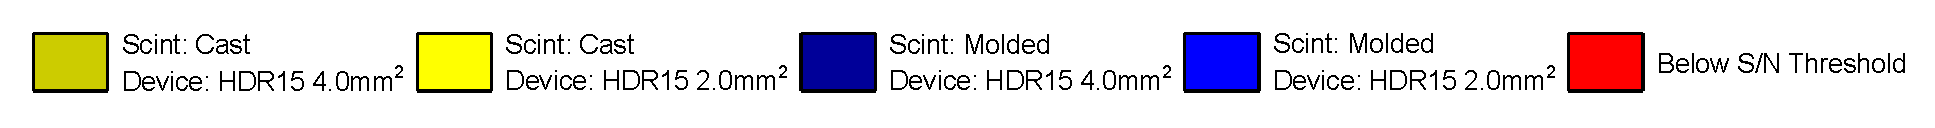
\includegraphics[width=\textwidth]{figures/hgcal/scenes_legend.pdf}
  \begin{minipage}[c]{0.49\textwidth}
    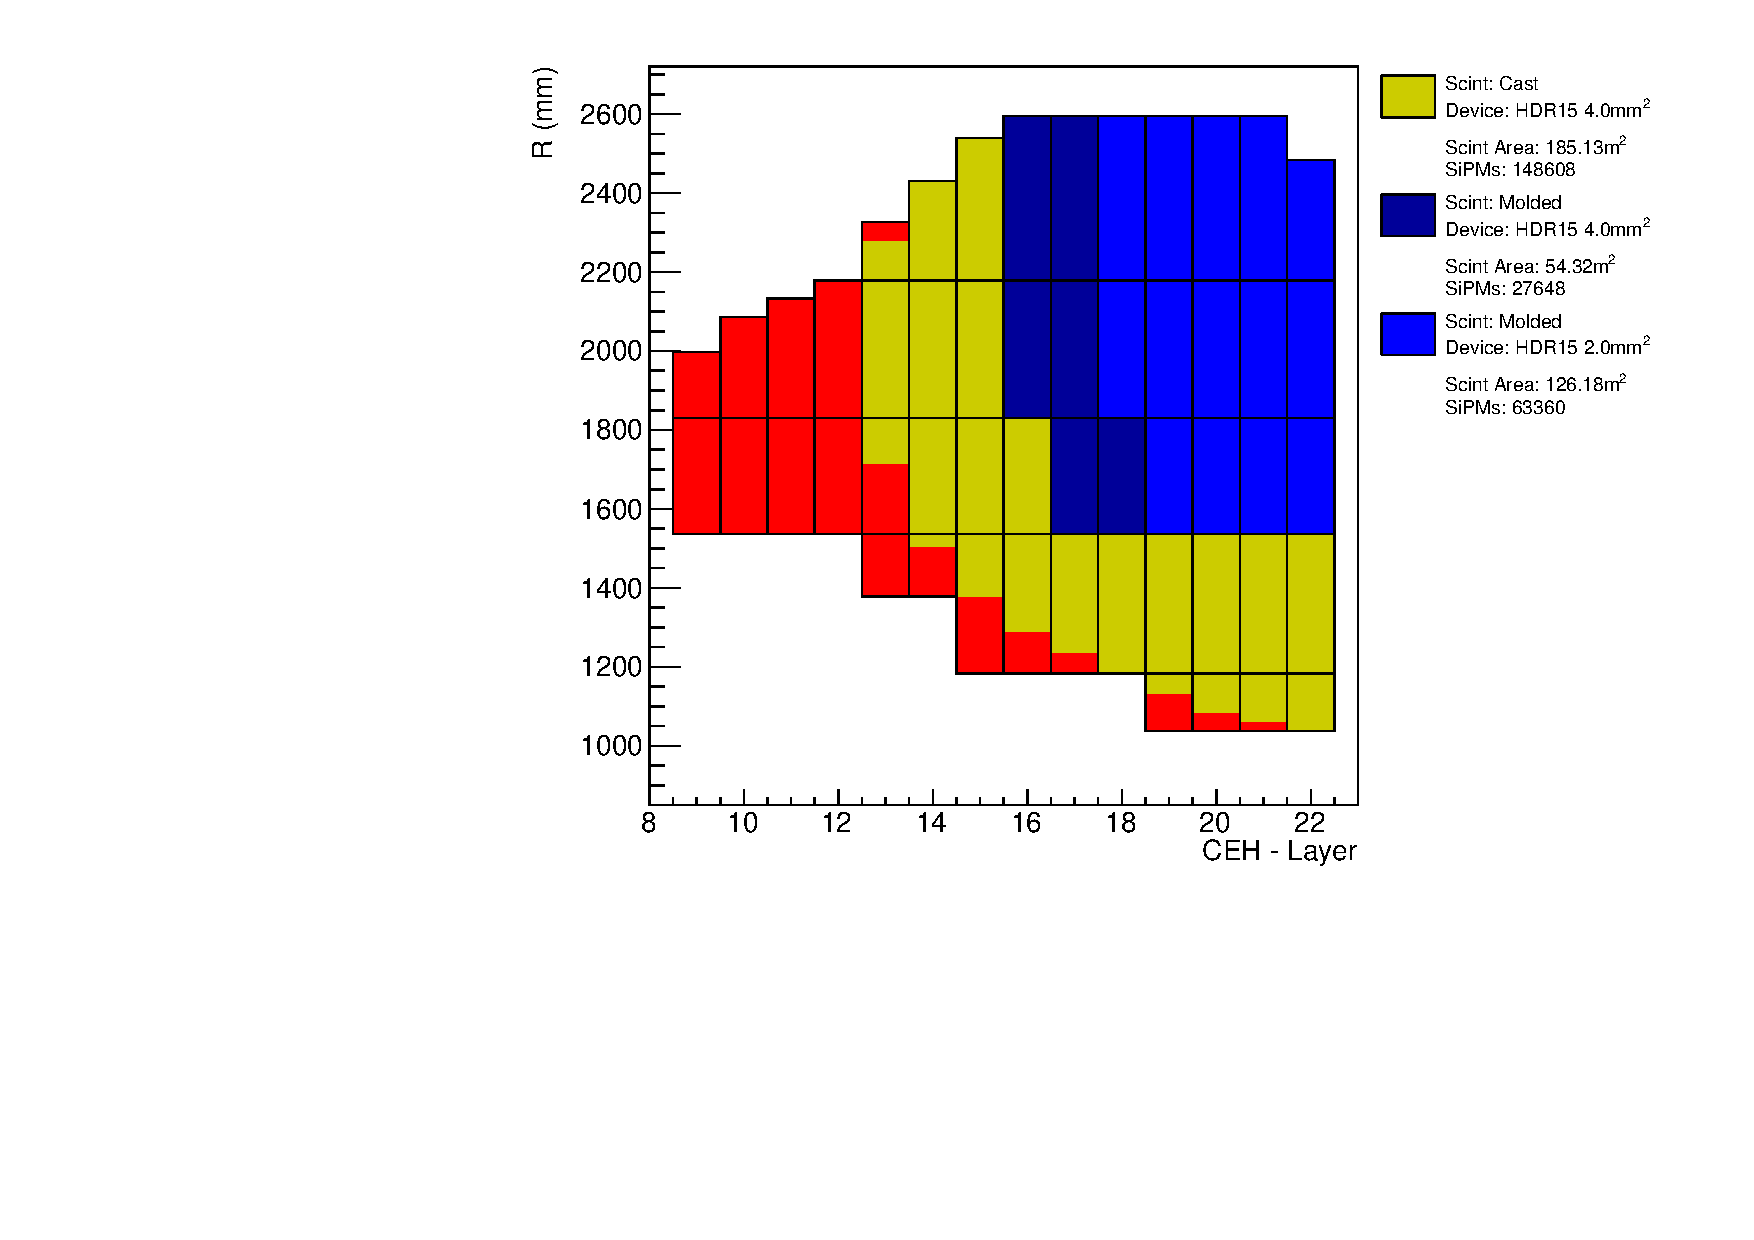
\includegraphics[trim={0 0 165pt 0},clip,width=\textwidth]{figures/hgcal/sceneA_jan20_2.pdf}
  \end{minipage}
  \begin{minipage}[c]{0.49\textwidth}
    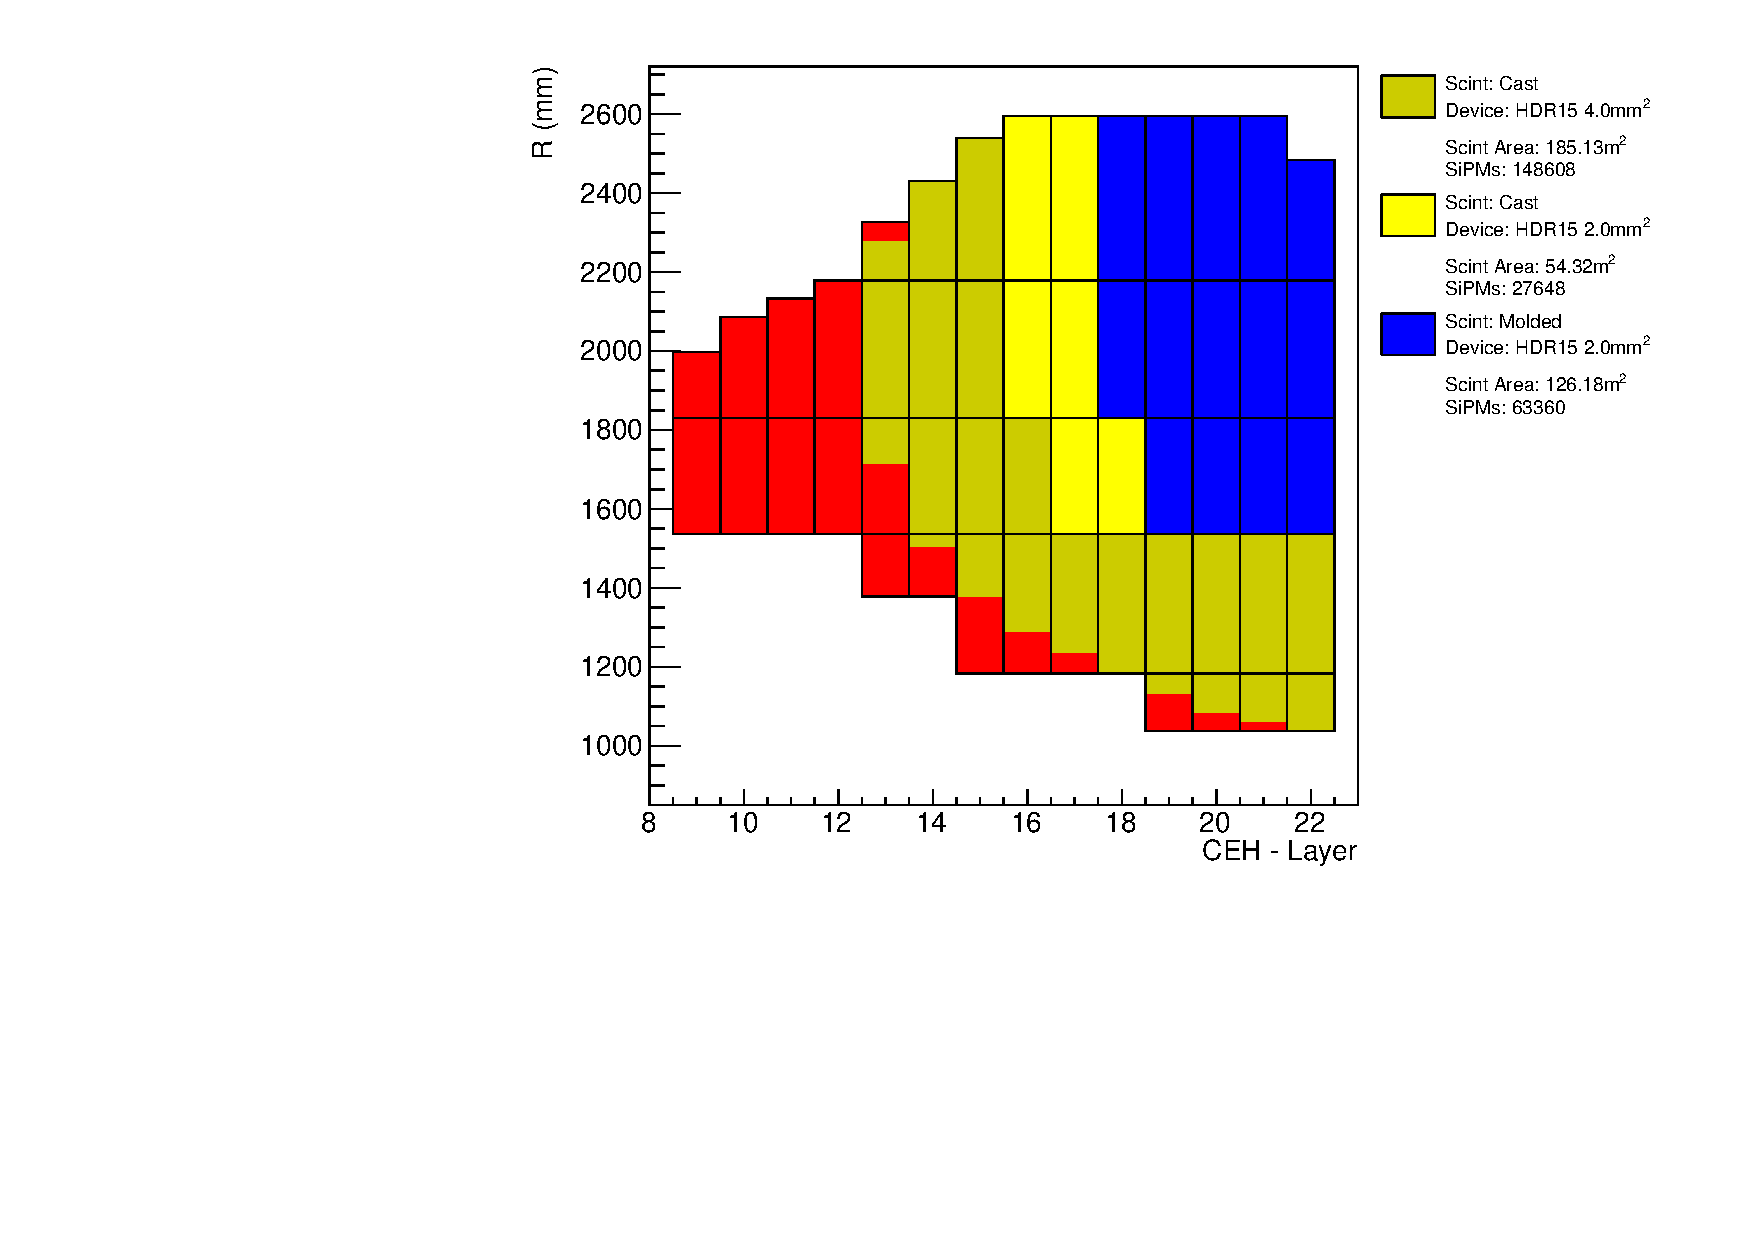
\includegraphics[trim={0 0 165pt 0},clip,width=\textwidth]{figures/hgcal/sceneB_jan20_2.pdf}
  \end{minipage}
  \caption[\gls{HGCAL} scenarios]{\gls{HGCAL} scenarios}%
  \label{fig:hgcal-scenes-fnal-jan20}
\end{figure}

\begin{table}[!ht]
  \centering
  \caption{\gls{HGCAL} scenarios comparison}
  \begin{tabular}{p{1.5in}cll}%
    \toprule
                                                   &                    & Scene A                & Scene B                \\
    \midrule
    \multirow{3}{=}{Cast Scintillator}             & Cell Count         & 148, 608               & 176, 256               \\
                                                   & Total Area         & 185.13 \(\text{m}^2 \) & 239.45 \(\text{m}^2 \) \\
                                                   & Percentage         & 50.6 \%                & 65.5 \%                \\
    \cmidrule(lr){2-4}
    \multirow{3}{=}{Injection Molded Scintillator} & Cell Count         & 91, 008                & 63, 360                \\
                                                   & Total Area         & 180.5 \(\text{m}^2 \)  & 126.18 \(\text{m}^2 \) \\
                                                   & Percentage         & 49.4 \%                & 34.5 \%                \\
    \cmidrule(lr){2-4}
    \multirow{2}{=}{SiPMs Count}                   & 2 \(\text{mm}^2 \) & 63, 360                & 91, 008                \\
                                                   & 4 \(\text{mm}^2 \) & 100, 224               & 148, 608               \\
    \bottomrule
  \end{tabular}
\end{table}